% =====================================================================
% SUPPLEMENTARY NOTE 7 — the claims axis, protocol by protocol.
%
% SOURCES. The ledger is Paper_writing/CLAIMS_LEDGER.md, built from the
% ten corpus papers' own PDFs; the protocols are EXPERIMENTS.md; every
% number in a table below is read from axw1008/docs/paper/x*.csv or the
% X3 run log by figures/scripts/supp_figures.py. Nothing here is a new
% calculation; it is the existing results laid out so each test can be
% read against the claim it answers.
%
% REGISTER. These are the sections' own numbers at full length. The
% Results subsection "Immune genes identify endometriosis" carries the
% pooled headline for each; this is where the per-protocol detail lives.
% =====================================================================

\section{The claims axis, protocol by protocol}
\label{note:claims}

Eleven studies were pooled to build this atlas, and ten of them made
claims about endometriosis from their own cohorts. None of the ten could
test another's, because no two share donors or a cell vocabulary. The
claims axis asks which of those claims the pooled corpus can settle, and
settles the ones it can. This note gives the ledger of claims, then each
test as a protocol with its full table, in the order the tests depend on
one another. The label transfer every composition test rests on is
Supplementary Note~\ref{note:transfer}; the marker-signature test is
Supplementary Note~\ref{note:markers}.

\subsection{The ledger}

Table~\ref{stab:ledger} lists every claim that bears on the disease, with
the cohort it was made from, the test applied here and the outcome. Claims
were taken from the papers themselves rather than from any review of them.
Three kinds of claim are outside the axis and are listed so that the
boundary is visible: claims about cell types finer than the four families,
which would need a finer transferred vocabulary; claims at the resolution
of a single pathway, which the forty-four groups merge
(Supplementary Note~\ref{note:limitations}); and claims from the one cohort
whose controls are not in the corpus.

\begin{table}[p]
\centering
\caption[The claims ledger]{\textbf{Published claims about endometriosis
from the corpus studies, and what the pooled corpus does with each.} Donor
counts are the cohort the claim was made from and the donors the test here
used.}
\label{stab:ledger}
\footnotesize\setlength{\tabcolsep}{3pt}
\begin{tabular}{@{}p{40mm}p{30mm}p{38mm}p{44mm}@{}}
\toprule
claim & source, donors & test here, donors & outcome \\
\midrule
eutopic endometrium of patients is transcriptionally altered & \texttt{duempelmann\_2026}, 60;\newline \texttt{tan\_2022}, 31 & cross-donor disease agreement, 207 donor records & supported: 0.3364, $P = 0.005$ \\
composition barely differs between patients and controls once phase is accounted for & \texttt{duempelmann\_2026}, 60 & X8, per-donor composition, 194 & supported: no family moves, $P \geq 0.24$ \\
severity is a dose: severe disease gives five times the differentially expressed genes of mild & \texttt{duempelmann\_2026}, 60 & latent severity among patients, 57; composition among patients, 51 & not recoverable at this donor count, in either readout; a different quantity, not a contradiction \\
macrophages and decidualised stromal cells are the compartments most likely dysregulated & \texttt{marecko\_2024}, 58,\newline from GWAS & X12, held-out disease direction within each family, 85 to 114 & immune half supported, 0.7084 at $P = 0.015$; stromal half not recoverable, 0.5920 at $P = 0.175$ \\
prior atlases lack reproducible marker signatures & \texttt{marecko\_2024} & X13, Supplementary Note~\ref{note:markers} & not supported on the marker half: 61 to 76 of each family's top hundred reproduce \\
disease abolishes the cyclical variation of immune composition & \texttt{lin\_2023}\newline (Huang), 13 & X3, cycle agreement by disease, 112; X3b, phase-by-disease interaction on composition, 101 & not supported in either test \\
composition differs between lesion and eutopic tissue & \texttt{ferrero\_2024}\newline (Sarsenova), 4 pairs & X9, per-donor composition by tissue, 151 & one family moves, epithelial 6.6-fold lower, confounded with dissociation; perivascular not resolvable \\
the same cell type differs transcriptionally by tissue site & \texttt{fonseca\_2023}, 48 & X14, tissue within a transferred family, 262 & weak residue in stromal and endothelial, $P = 0.08$ and $0.10$; tissue is a decoder covariate \\
lesions carry a less differentiated, progenitor-like epithelium & \texttt{garcia\_alonso\_2021}\newline (bulk deconvolution);\newline \texttt{tan\_2022}, 14 & needs epithelial subtypes & not tested; 58 ectopic donors available \\
four case-against-control findings, two at $P < 10^{-16}$ & \texttt{shih\_2022}, 11 here & none possible & untestable: no controls in the deposited cohort \\
metabolic reprogramming in named pathways; steroid signalling; iron and senescence & \texttt{ferrero\_2024};\newline \texttt{li\_2025} & needs single-pathway resolution & not tested; the groups merge the pathways named \\
perivascular and mural cell findings in three cohorts & \texttt{duempelmann\_2026},\newline \texttt{tan\_2022},\newline \texttt{ferrero\_2024} & needs a finer vocabulary & future work \\
\bottomrule
\end{tabular}
\end{table}

\subsection{X3: the cycle in the latent, by disease status}

The claim is that in controls the proportions of immune cells vary across
the menstrual cycle and in endometriosis that variation disappears
\citep{huang2023immune}, made from thirteen donors. The first test asks the
latent: cross-donor cycle agreement was computed separately over control
donors and over eutopic donors, with a permutation null for the difference
built by reassigning disease status across donors. The held-out restriction
was dropped for this test because the phase head is one linear map from
latent position to phase and cannot store which donor had which phase, and
because training donors scored no higher than held-out ones, 0.6422 against
0.6545; keeping the restriction would have cost two thirds of the donors
for nothing. Over 112 donors the control excess is 0.6825 and the eutopic
0.7474, a difference of $-0.0650$ against a null spanning $-0.1802$ to
$+0.1949$, $P = 0.505$ (Tables~\ref{stab:x3} and~\ref{stab:x3d}). The
claim predicts a positive difference; the measured one is small and
negative, and the null is narrow enough that a difference of the size
claimed would have been seen. Phase labels come from three studies, so this
is a three-cohort result rather than a corpus-wide one.

\begin{table}[t]
\centering
\caption[X3, cycle agreement by disease]{\textbf{Cross-donor cycle
agreement among control donors and among eutopic donors.}}
\label{stab:x3}
\small
% GENERATED by figures/scripts/supp_figures.py. Do not edit by hand.
\begin{tabular}{@{}lrrrrrr@{}}
\toprule
donors & n & cells & phases & agreement & chance & excess \\
\midrule
control & 61 & 307{,}040 & 8 & 0.7600 & 0.2443 & 0.6825 \\
eutopic & 51 & 318{,}936 & 6 & 0.8052 & 0.2288 & 0.7474 \\
\bottomrule
\end{tabular}

\end{table}

\begin{table}[t]
\centering
\caption[X3, the difference and its null]{\textbf{The difference between
the two groups and its permutation null.}}
\label{stab:x3d}
\small
% GENERATED by figures/scripts/supp_figures.py. Do not edit by hand.
\begin{tabular}{@{}lr@{}}
\toprule
quantity & value \\
\midrule
control minus eutopic, excess & $-$0.0650 \\
null mean & 0.0018 \\
null s.d. & 0.0961 \\
null 95\% interval & $-$0.1802 to 0.1949 \\
two-sided $P$ & 0.505 \\
permutations & 2{,}000 \\
\bottomrule
\end{tabular}

\end{table}

\subsection{X3b: the same claim, as the source made it}

The claim is about proportions, not latent geometry, so the second test
uses no model output. For each of 101 donors carrying a family label, a
phase and a disease status, the immune share of cells was fitted as
$\mathrm{logit}(\text{share}) \sim \text{study} + \text{phase} +
\text{disease} + \text{phase} \times \text{disease}$. The interaction term
is the claim written as arithmetic. The null permutes disease status across
donors within study, keeping each donor's phase and composition together,
5{,}000 times. The interaction $F$ is 0.263 against a null whose 95th
percentile is 3.061, $P = 0.762$ (Table~\ref{stab:x3b}). The two tests use
different instruments, one the representation and one a headcount, and
agree; the second cannot be attributed to anything the model does.

\begin{table}[t]
\centering
\caption[X3b, the interaction test]{\textbf{The phase-by-disease interaction
on immune composition}, 101 donors, study as a covariate.}
\label{stab:x3b}
\small
% GENERATED by figures/scripts/supp_figures.py. Do not edit by hand.
\begin{tabular}{@{}lr@{}}
\toprule
quantity & value \\
\midrule
donors & 101 \\
interaction $F$, phase $\times$ disease & 0.263 \\
null mean $F$ & 0.996 \\
null 95th percentile & 3.061 \\
$P$ & 0.762 \\
permutations & 5{,}000 \\
\bottomrule
\end{tabular}

\end{table}

\subsection{X8: composition, control against eutopic}

The claim is that, stratified by phase, cell composition barely differs
between patients and controls, with one exception among 57 cell types
\citep{duempelmann2026endometrium}, made from 60 donors. For each of 194
donors with endometrium in the corpus, the share of each family was
computed over the transferred and annotated labels together, and disease
status was tested after study with a permutation null of 5{,}000
reassignments within study. No family moves: $P = 0.6186$ for immune cells,
0.7360 stromal, 0.9016 epithelial and 0.2358 endothelial
(Table~\ref{stab:x8}, Supplementary Fig.~\ref{sfig:comp-ce}). The raw means
differ, 0.101 against 0.230 for the immune share, and the difference does
not survive study being accounted for, which is the pooling doing what it
is for. The four shares sum to one and the families were named in advance,
so these are not four independent attempts.

\begin{table}[t]
\centering
\caption[X8, composition by disease status]{\textbf{Per-donor cell-family
share, control against eutopic endometrium}, 194 donors.}
\label{stab:x8}
\small
% GENERATED by figures/scripts/supp_figures.py. Do not edit by hand.
\begin{tabular}{@{}lrrrr@{}}
\toprule
family & mean share, control & mean share, eutopic & $F$ & $P$ \\
\midrule
stromal & 0.523 & 0.584 & 0.125 & 0.7360 \\
epithelial & 0.331 & 0.147 & 0.017 & 0.9016 \\
endothelial & 0.046 & 0.039 & 1.445 & 0.2358 \\
immune & 0.101 & 0.230 & 0.249 & 0.6186 \\
\bottomrule
\end{tabular}

\end{table}

\begin{figure}[t]
\centering
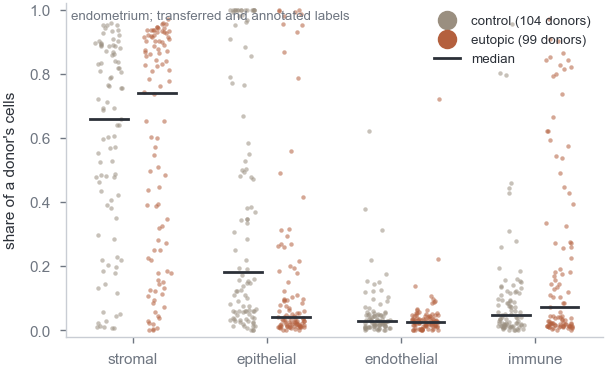
\includegraphics[width=.65\textwidth]{figures/composition_control_vs_eutopic.png}
\caption[Composition, control against eutopic]{\textbf{Each donor's share
of each family, control against eutopic endometrium.} Bars are medians.}
\label{sfig:comp-ce}
\end{figure}

\subsection{X8, extended: composition against severity}

Among patients only, donors were split into lower severity, graded mild or
rASRM stage I to II, and higher, graded severe or stage III to IV, 51
donors, and the same test run. Nothing tracks severity: $P = 0.2092$ for
immune cells, 0.1624 endothelial, 0.9696 stromal and 0.9130 epithelial
(Table~\ref{stab:x8sev}, Supplementary Fig.~\ref{sfig:comp-sev}). Beside
the latent result, where merged severity clears its null at 118 donors and
mild against severe among patients does not at 57, this is a second and
independent readout failing on the same contrast, one from the
representation and one from a headcount with no model in it. Both are
negatives at about 55 donors, so the pairing is the argument rather than
either number alone.

\begin{table}[t]
\centering
\caption[X8, composition by severity]{\textbf{Per-donor cell-family share
by surgical severity, patients only}, 51 donors.}
\label{stab:x8sev}
\small
% GENERATED by figures/scripts/supp_figures.py. Do not edit by hand.
\begin{tabular}{@{}lrrrr@{}}
\toprule
family & mean share, low severity & mean share, high severity & $F$ & $P$ \\
\midrule
stromal & 0.702 & 0.791 & 0.002 & 0.9696 \\
epithelial & 0.178 & 0.150 & 0.012 & 0.9130 \\
endothelial & 0.029 & 0.028 & 2.038 & 0.1624 \\
immune & 0.091 & 0.031 & 1.620 & 0.2092 \\
\bottomrule
\end{tabular}

\end{table}

\begin{figure}[t]
\centering
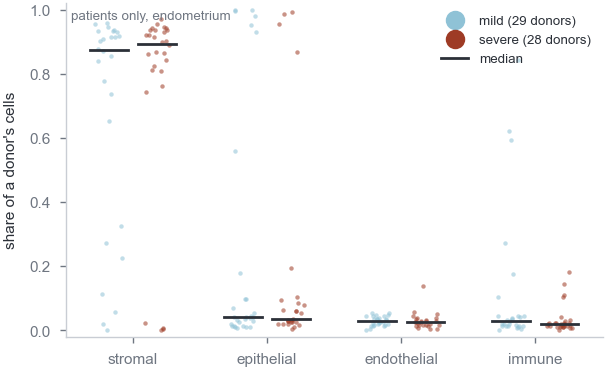
\includegraphics[width=.65\textwidth]{figures/composition_by_severity.png}
\caption[Composition by severity]{\textbf{Each patient's share of each
family, by severity grade.} The figure draws every patient carrying a
grade; the test used the 51 with the required covariates.}
\label{sfig:comp-sev}
\end{figure}

\subsection{X9: composition, eutopic against lesion}

The claim is that perivascular, endothelial and immune cells form a larger
share of lesions and stromal cells a smaller one
\citep{sarsenova2024metabolic}, from four paired samples. Over 151 donors,
one family moves: the epithelial share falls from 0.147 in eutopic
endometrium to 0.022 in lesion tissue, 6.6-fold, $F = 20.9$,
$P < 0.0001$; immune, endothelial and stromal do not clear
(Table~\ref{stab:x9}, Supplementary Fig.~\ref{sfig:comp-ee}). The direction
agrees with the claim. The source names the confound: epithelial cells are
lost when fibrous lesion tissue is dissociated, and nothing in the corpus
separates that from biology. The label-absorption error of
Supplementary Note~\ref{note:transfer} would push the epithelial share in
lesions up rather than down, so it does not manufacture this result.
Perivascular cells are not one of the four families and the claim's central
compartment is out of reach.

\begin{table}[t]
\centering
\caption[X9, composition by tissue]{\textbf{Per-donor cell-family share,
eutopic endometrium against lesion tissue}, 151 donors.}
\label{stab:x9}
\small
% GENERATED by figures/scripts/supp_figures.py. Do not edit by hand.
\begin{tabular}{@{}lrrrr@{}}
\toprule
family & mean share, eutopic & mean share, ectopic & $F$ & $P$ \\
\midrule
stromal & 0.584 & 0.496 & 0.044 & 0.8180 \\
epithelial & 0.147 & 0.022 & 20.895 & $<$ 0.0001 \\
endothelial & 0.039 & 0.080 & 0.208 & 0.7002 \\
immune & 0.230 & 0.401 & 2.864 & 0.1194 \\
\bottomrule
\end{tabular}

\end{table}

\begin{figure}[t]
\centering
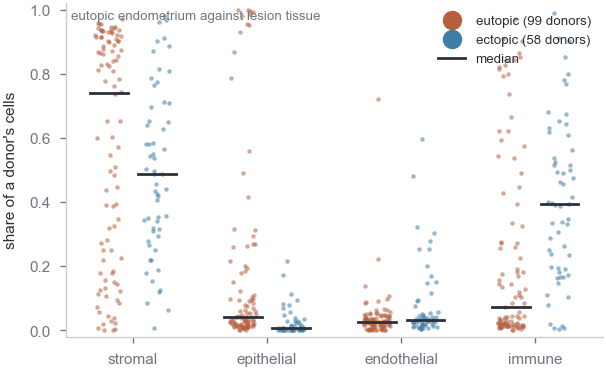
\includegraphics[width=.65\textwidth]{figures/composition_eutopic_vs_ectopic.png}
\caption[Composition, eutopic against lesion]{\textbf{Each donor's share
of each family, eutopic endometrium against lesion tissue.}}
\label{sfig:comp-ee}
\end{figure}

\subsection{X12, step A: where in the latent the disease lives}

The claim is that macrophages and decidualised stromal cells are the
compartments most likely dysregulated in endometriosis, derived by
integrating an atlas with the largest endometriosis GWAS
\citep{mareckova2024heca}. The test looks for a direction in the latent
that separates control donors from eutopic donors, fitted on 70\% of donors
and scored by AUC on the remaining 30\%, repeated over 400 donor-level
splits, with a shuffled-label null; study is centred out and donors rather
than cells are the units. Globally no such direction exists: 0.5360
against a shuffled 0.4820 over 207 donor records, with 28\% of shuffles
above it (Table~\ref{stab:x12g}). That does not contradict the cross-donor
disease figure, which is local; a cell's neighbours from other donors can
share its label without any single axis separating the donors.

Inside each family, over the 118 donors with the studies' own labels, the
direction appears and it is immune: AUC 0.7084 against 0.4806,
$P = 0.015$ over 94 donors; endothelial 0.6818 at $P = 0.050$; stromal
0.5920 at 0.175; epithelial 0.4663 at 0.590; and the four families pooled
0.6048 at 0.155 (Table~\ref{stab:x12a},
Supplementary Fig.~\ref{sfig:x12-auc-a}). Mixing the families destroys a
signal that is present inside one of them. Four families were tested, so a
Bonferroni correction puts immune at about 0.06 and endothelial at 0.20;
immune is the only compartment worth calling and it is real rather than
emphatic. On the transferred labels over 207 donor records the pattern
holds and weakens, immune 0.5960 at $P = 0.072$ over 162
(Table~\ref{stab:x12t}, Supplementary Fig.~\ref{sfig:x12-auc-t}); the
reason the paper reports 118 rather than 207 is given in
Supplementary Note~\ref{note:limitations}.

\begin{table}[t]
\centering
\caption[X12, the global direction]{\textbf{The global control-against-case
direction}, fitted and scored across donor-level splits.}
\label{stab:x12g}
\small
% GENERATED by figures/scripts/supp_figures.py. Do not edit by hand.
\begin{tabular}{@{}lr@{}}
\toprule
quantity & value \\
\midrule
donor records & 207 \\
held-out AUC, global direction & 0.5360 \\
shuffled-label AUC & 0.4820 \\
share of shuffles above observed & 0.28 \\
cosine stability of the direction across splits & 0.8526 \\
\bottomrule
\end{tabular}

\end{table}

\begin{table}[t]
\centering
\caption[X12, direction within each family, own labels]{\textbf{The
disease direction within each family, studies' own labels}, 118 donors.
Interval is the 2.5th to 97.5th percentile over 400 splits.}
\label{stab:x12a}
\footnotesize
% GENERATED by figures/scripts/supp_figures.py. Do not edit by hand.
\begin{tabular}{@{}lrrrrrr@{}}
\toprule
compartment & donors & ctl / case & held-out AUC & 95\% interval & shuffled AUC & $P$ \\
\midrule
all families, pooled & 114 & 60 / 54 & 0.6048 & 0.454 to 0.750 & 0.5028 & 0.155 \\
stromal & 101 & 54 / 47 & 0.5920 & 0.437 to 0.753 & 0.4986 & 0.175 \\
epithelial & 98 & 51 / 47 & 0.4663 & 0.304 to 0.632 & 0.4898 & 0.590 \\
immune & 94 & 50 / 44 & 0.7084 & 0.566 to 0.856 & 0.4806 & 0.015 \\
endothelial & 85 & 43 / 42 & 0.6818 & 0.523 to 0.827 & 0.4864 & 0.050 \\
\bottomrule
\end{tabular}

\end{table}

\begin{table}[t]
\centering
\caption[X12, direction within each family, transferred labels]{\textbf{The
same test over 207 donor records with transferred labels.}}
\label{stab:x12t}
\footnotesize
% GENERATED by figures/scripts/supp_figures.py. Do not edit by hand.
\begin{tabular}{@{}lrrrrrr@{}}
\toprule
compartment & donors & ctl / case & held-out AUC & 95\% interval & shuffled AUC & $P$ \\
\midrule
all families, pooled & 202 & 106 / 96 & 0.5176 & 0.411 to 0.624 & 0.4710 & 0.268 \\
stromal & 175 & 86 / 89 & 0.4921 & 0.379 to 0.610 & 0.4804 & 0.445 \\
epithelial & 176 & 93 / 83 & 0.4701 & 0.338 to 0.581 & 0.4780 & 0.535 \\
immune & 162 & 76 / 86 & 0.5960 & 0.471 to 0.711 & 0.4821 & 0.072 \\
endothelial & 134 & 65 / 69 & 0.5947 & 0.481 to 0.709 & 0.4782 & 0.102 \\
\bottomrule
\end{tabular}

\end{table}

\begin{figure}[t]
\centering
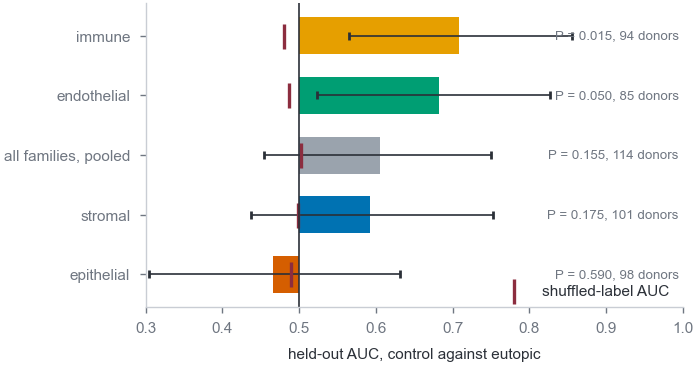
\includegraphics[width=.65\textwidth]{figures/x12_auc_by_family_annotated.png}
\caption[Disease AUC by family, own labels]{\textbf{Held-out AUC of the
disease direction within each family and pooled}, studies' own labels,
with the shuffled-label value marked.}
\label{sfig:x12-auc-a}
\end{figure}

\begin{figure}[t]
\centering
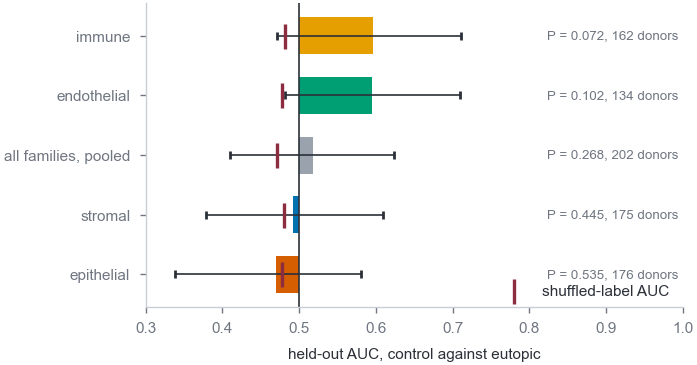
\includegraphics[width=.65\textwidth]{figures/x12_auc_by_family_transferred.png}
\caption[Disease AUC by family, transferred labels]{\textbf{The same,
over 207 donor records with transferred labels.}}
\label{sfig:x12-auc-t}
\end{figure}

\subsection{X12, step B: the genes the immune direction moves}

The immune direction was pushed through the decoder: 4{,}000 immune cells
were moved along it and the change in every one of the 15{,}496 decoded
genes recorded, after the component of the direction lying along the
family axes was removed. The ranking is stable in the step size, with a rank
correlation of 0.9973 between two step lengths. Table~\ref{stab:x12top}
gives the fifteen genes that move most towards disease and
Table~\ref{stab:x12bot} the fifteen that move most towards control;
Supplementary Fig.~\ref{sfig:x12-rank} draws the whole ranking. The
disease end is macrophage and inflammatory transcripts, TREM1, IL1B, CCL13,
SIGLEC7, the matrix proteases MMP19 and MMP27, LRRC15 and INHBA, with CCL3
at rank 52 and ITGAX at 47 just outside the table.

Three external readings bear on it. An independent cohort outside the
corpus, eight patients against five controls, published 66 genes
upregulated in the eutopic endometrium of patients
\citep{zhao2017transcriptome}; four of the fifteen disease-end genes are on
that list, SERPINB2 at 72.95-fold, MMP27 at 40.93, LRRC15 at 25.20 and INHBA
at 15.33, a hypergeometric $P$ of $3.95 \times 10^{-7}$ for fifteen draws
from 15{,}496, and none of the fifteen control-end genes is
(Table~\ref{stab:x12rep}). IL1B, tenth here, is the highest-ranked gene in
\texttt{duempelmann\_2026}'s own supervised classifier of disease, so two
models with different objectives select it, and CCL3 and ITGAX appear in
that cohort's ligand-receptor findings as well
\citep{duempelmann2026endometrium}. Of the four gene-level predictions of
the prior atlas, only IGF1 rising in macrophages is a claim about this
compartment, and it agrees, at rank 285 of 15{,}496 towards disease; GREB1,
DKK1 and IGF2 are predictions about decidualised stromal cells, and there is
no stromal direction to test them on. The control end is led by genes of
epithelial identity and secretory function, VTCN1, SOX17, IHH and UGT2B17,
with WNT7A, LGR5, MSLN and TFF3 inside the last 220 of the ranking; that end
is not read as disease biology and replicates nothing. Four of the fifteen
disease-end genes, SIGLEC7, ADAMDEC1, ALPK2 and KCNH1, have no prior
endometriosis report in the eleven pooled studies, the Open Targets
Platform or PubMed. Two of the genes that do replicate, LRRC15 and MMP27,
are absent from one or both of those indices despite being reported at
25- and 41-fold in the external cohort's supplementary tables, so absence
from an index is not evidence of novelty and the four are reported as
unindexed rather than as new.

\begin{table}[p]
\centering
\caption[X12, the disease end of the ranking]{\textbf{The fifteen genes
moving most towards disease along the immune direction.}}
\label{stab:x12top}
\footnotesize
% GENERATED by figures/scripts/supp_figures.py. Do not edit by hand.
\begin{tabular}{@{}rlrrl@{}}
\toprule
rank & gene & shift towards disease & external up-list, fold & indexed report \\
\midrule
1 & LRRC15 & 0.0733 & 25.20 &  \\
2 & TREM1 & 0.0620 & -- &  \\
3 & SCARA5 & 0.0616 & -- &  \\
4 & CCL13 & 0.0608 & -- &  \\
5 & CST11 & 0.0606 & -- &  \\
6 & SIGLEC7 & 0.0594 & -- & none found \\
7 & KCNH1 & 0.0592 & -- & none found \\
8 & DKK1 & 0.0571 & -- &  \\
9 & SERPINB2 & 0.0569 & 72.95 &  \\
10 & IL1B & 0.0567 & -- &  \\
11 & MMP19 & 0.0566 & -- &  \\
12 & MMP27 & 0.0559 & 40.93 &  \\
13 & ADAMDEC1 & 0.0556 & -- & none found \\
14 & INHBA & 0.0555 & 15.33 &  \\
15 & ALPK2 & 0.0550 & -- & none found \\
\bottomrule
\end{tabular}

\end{table}

\begin{table}[p]
\centering
\caption[X12, the control end of the ranking]{\textbf{The fifteen genes
moving most towards control along the same direction.}}
\label{stab:x12bot}
\small
% GENERATED by figures/scripts/supp_figures.py. Do not edit by hand.
\begin{tabular}{@{}rlr@{}}
\toprule
rank & gene & shift towards control \\
\midrule
1 & PLP1 & 0.0670 \\
2 & AMIGO3 & 0.0644 \\
3 & INS & 0.0622 \\
4 & UGT1A5 & 0.0598 \\
5 & NPY2R & 0.0581 \\
6 & SLIT2 & 0.0578 \\
7 & CFHR4 & 0.0577 \\
8 & NPAP1 & 0.0547 \\
9 & DCLK1 & 0.0539 \\
10 & EPHA5 & 0.0533 \\
11 & EBF2 & 0.0531 \\
12 & ADGRB3 & 0.0525 \\
13 & LRRC15 & 0.0523 \\
14 & COL6A6 & 0.0519 \\
15 & HTN1 & 0.0517 \\
\bottomrule
\end{tabular}

\end{table}

\begin{table}[t]
\centering
\caption[X12, external replication]{\textbf{Overlap of each end of the
ranking with an external cohort's upregulated list.}}
\label{stab:x12rep}
\footnotesize
\resizebox{\textwidth}{!}{% GENERATED by figures/scripts/supp_figures.py. Do not edit by hand.
\begin{tabular}{@{}lrrrrl@{}}
\toprule
end of the ranking & genes taken & external list & hits & hypergeometric $P$ & genes \\
\midrule
disease side & 15 & 66 upregulated & 4 & $3.95\times10^{-7}$ & INHBA, LRRC15, MMP27, SERPINB2 \\
control side & 15 & 66 upregulated & 0 & 1.0 & -- \\
\bottomrule
\end{tabular}
}
\end{table}

\begin{figure}[t]
\centering
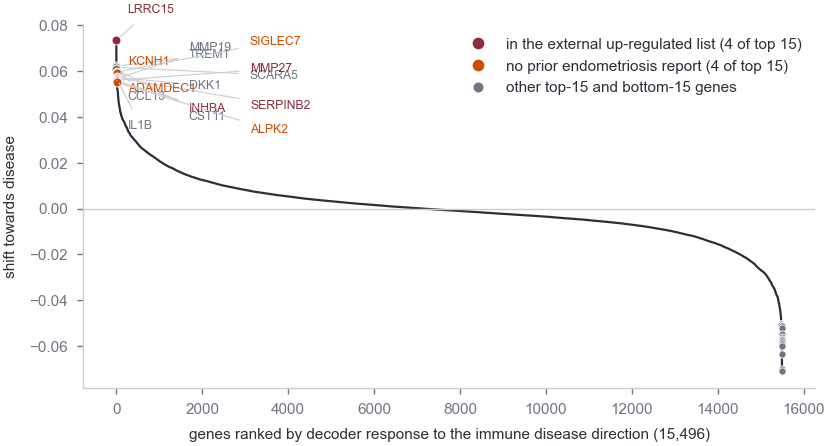
\includegraphics[width=.9\textwidth]{figures/x12_gene_ranking.png}
\caption[The gene ranking along the immune direction]{\textbf{All
15{,}496 genes ranked by decoder response to the immune disease direction.}
The four externally replicating genes and the four unindexed genes are
marked at the disease end; the control end replicates nothing.}
\label{sfig:x12-rank}
\end{figure}

\subsection{X14: tissue inside one family}

The claim is that the same cell type is transcriptionally different
depending on the tissue it sits in \citep{fonseca2023endometriosis}.
Tissue is a decoder covariate, which conditions the test rather than
invalidating it: conditioning the decoder on tissue removes the latent's
obligation to encode it, so tissue structure that survives in the latent is
structure the model had every reason to discard. Within each transferred
family, (donor, tissue) units were scored for endometrium against lesion
tissue after study, 262 donors, with donor-level splits and a shuffled null.
Most tissue structure is gone; what remains sits in stromal and endothelial
cells, AUC 0.6226 at $P = 0.077$ and 0.6175 at 0.095, with immune and
epithelial at chance (Table~\ref{stab:x14},
Supplementary Fig.~\ref{sfig:x14}). Tissue is near-perfectly confounded
with disease status here, since ovary and peritoneum are almost all ectopic
donors, so this is the latent-level companion to X9 rather than an
independent axis, and neither family clears 0.05.

\begin{table}[t]
\centering
\caption[X14, tissue within a family]{\textbf{Endometrium against lesion
tissue within each transferred family}, 262 donors.}
\label{stab:x14}
\small
% GENERATED by figures/scripts/supp_figures.py. Do not edit by hand.
\begin{tabular}{@{}lrrrrrr@{}}
\toprule
family & (donor, tissue) units & endometrium & lesion & AUC & shuffled AUC & $P$ \\
\midrule
stromal & 229 & 171 & 58 & 0.6226 & 0.4946 & 0.077 \\
epithelial & 194 & 173 & 21 & 0.5222 & 0.4936 & 0.401 \\
endothelial & 175 & 131 & 44 & 0.6175 & 0.4935 & 0.095 \\
immune & 215 & 158 & 57 & 0.5618 & 0.5019 & 0.240 \\
\bottomrule
\end{tabular}

\end{table}

\begin{figure}[t]
\centering
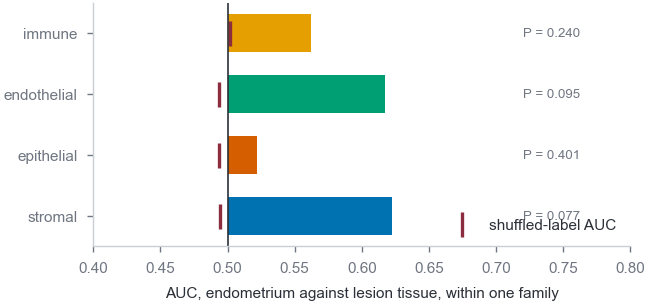
\includegraphics[width=.6\textwidth]{figures/x14_tissue_within_family.png}
\caption[Tissue within a family, drawn]{\textbf{Table~\ref{stab:x14}
drawn.}}
\label{sfig:x14}
\end{figure}
